\documentclass[ twoside,openright,titlepage,numbers=noenddot,headinclude,%1headlines,% letterpaper a4paper
                footinclude=true, cleardoublepage=empty,abstractoff, % <--- obsolete, remove (todo)
                BCOR=5mm,paper=a4,fontsize=11pt,%11pt,a4paper,%
                ]{scrreprt}
                
\usepackage{graphicx}
\graphicspath{ {images/gitLab/} }

\begin{document}

\chapter{gitlabUsage guide}
\section{Create new Project:}

\begin{itemize}
	\item go to website, create new Project, follow instructions, to the mkdirs in  your project directory
	\item Create SSHkey, to project
	\item \texttt{add remote add origin}
	\item \texttt{push -u origin master}    (the master branch is now the origin branch, all next pushes are going to this branch)
\end{itemize}

\section{define sshkeys}

\begin{enumerate}
\item \texttt{ssh-keygen -t rsa -C \"yourEmail\"} \#to create a ssh key in linux
\item cat /home/.ssh/id\_rsa.pub   \# shows the ssh key
\item ssh -T git@github.com  \#test the ssh and activate it
\item github to settings to deploy keys to Add deploy key
\end{enumerate}

if we have different git repositories we can make a config file in the 
~/.ssh/ folder
Host krios
HostName krios.tbi.univie.ac.at
IdentityFile ~/.ssh/id\_rsa\_krios

Host github.com
HostName github.com
IdentityFile ~/.ssh/id\_rsa\_github




\section{important commands}
\subsection{\texttt{git status}}
	show the status, what is already commit, what is new what is modified
\subsection{\texttt{git pull}}
	update your local folder
\subsection{\texttt{git diff} filename1}
	show the difference between the current file and the file in the repository
\subsection{\texttt{git rm}}
	removes a file from the git repository and from the file system, changes are recognized now by commit and push	
	
	if you removed a file from the disc but in githubm than you have to use git add -u filename to let git recognize it
\subsection{\texttt{git clone} SSH address project}
		copies an entire gitlab project to the current folder
\subsection{\texttt{git checkout} file1 }
		drop every change made with file1, and restore the information in the repository 
\section{change a file and add it to the repository }
	\begin{itemize}
		\item \texttt{git pull}
		\item \texttt{git status}
		\item \texttt{git diff} filename1
		\item \texttt{git add} filename1
		\item \texttt{git commit -m "your comment"}
		\item \texttt{git status}
		\item \texttt{git push} or \texttt{git push -u origin branchname1} if the commits should go to another branch
	\end{itemize}

\section{managing branches}
	\begin{itemize}
		\item \texttt{git branch}
			
			show all branches, and the current branch
		\item \texttt{git checkout} branchname1
			
			switch to branch branchname1
		\item \texttt{git checkout -b} newBranchName
		
			create new branch newBranchName
		\item \texttt{git push -u origin }newBranchName
			
			now commits will be pushed to this branch if \texttt{git push} was called
			
		\item \texttt{git branch -d branchName1}
			
			delete branch
		
		\item \texttt{git branch -m newname}
			
			rename current branch to newname
			
		\item \texttt{git rebase branch1}
		
			take the current branch and set it as head to branch1
			Caution: merges can occur
	\end{itemize}
\section{Get back in the git History, only working on local, not on repository(github cannot do this)}
	\begin{enumerate}
		\item \texttt{git log} (show all commits)
			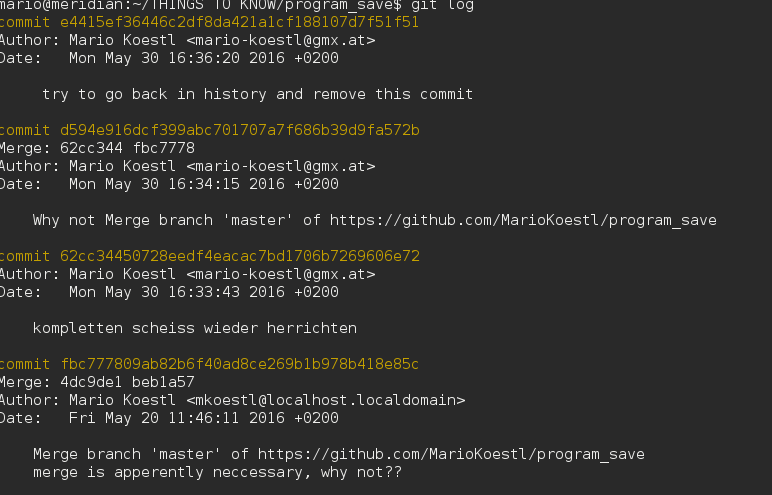
\includegraphics[width=8cm,height=8cm]{pictures/gitLog.png}
		\item \texttt{git format-patch} Hashkey  (of commitNode where we want to go back)
		
			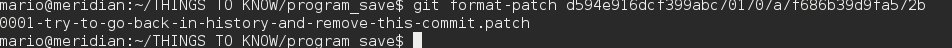
\includegraphics[scale=0.5]{pictures/patchFileCreated.png}
		\item \texttt{less} patchfile ( show the patchfile changes)
		
			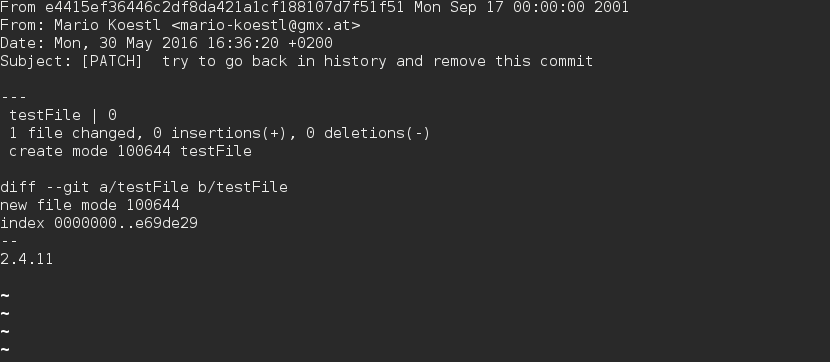
\includegraphics[width=8cm,height=8cm]{pictures/patchFile.png}
		\item \texttt{git reset --hard} hashkey (of commitNode where we want to go back)
		
			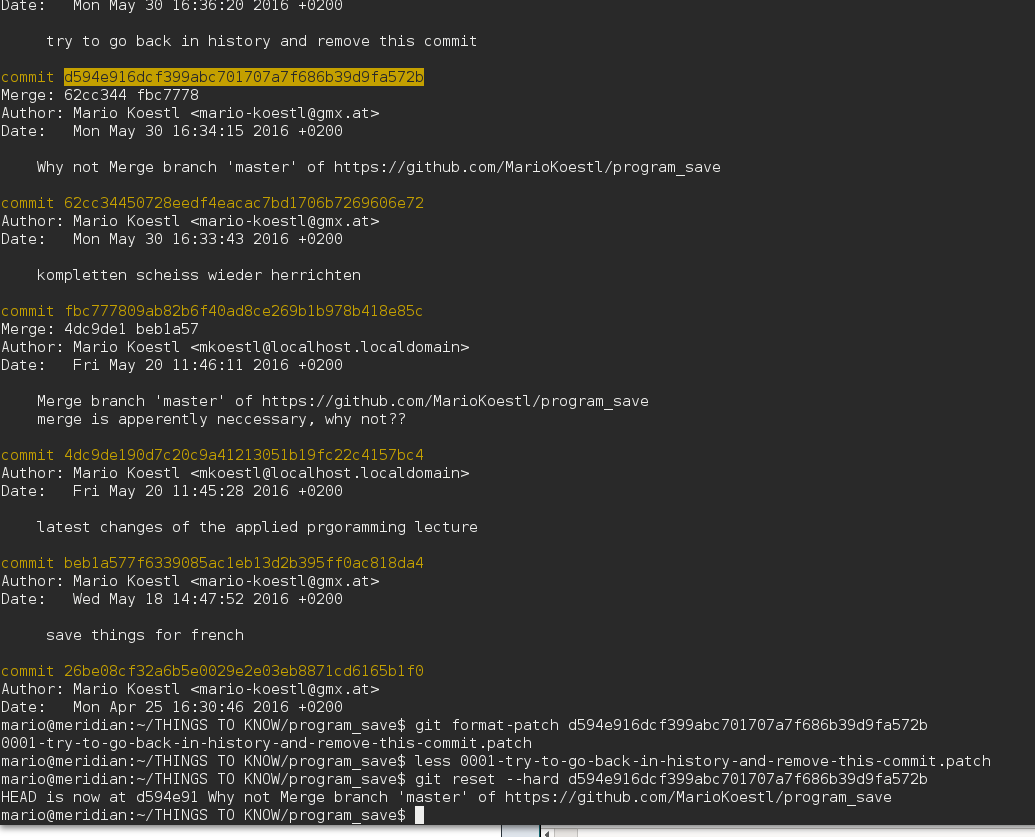
\includegraphics[width=8cm,height=8cm]{pictures/reseted.png}
		\item \texttt{patch -p1 < } patchfile 
		
			(undo saved changes, p1 if hirarchy is a/filename and b/filename,  else 2 or 3)
	\end{enumerate}

\end{document}